\chapter{ПРОЕКТИРОВАНИЕ СИСТЕМЫ УПРАВЛЕНИЯ ДВИЖЕНИЕМ БЕСПИЛОТНОГО АВТОМОБИЛЯ}
В данной главе рассматривается этап проектирования структуры и алгоритмов системы управления движением беспилотного
автомобиля. Проектирование системы основано на анализе рассмотренных архитектурных решений и алгоритмов.

\section{Формулирование требований к разрабатываемой системе}


Система управления беспилотным автомобилем должна выполнять большое количество функций, необходимых для эффективного
и безопасного движения в сложных условиях, среди которых
\begin{itemize}
    \item распознавание других участников дорожного движения (автомобилей, пешеходов,
          велосипедистов и т.п.);
    \item отслеживать других участников дорожного движения в течении некоторого времени для определения характеристик
          их движения и уменьшения ошибок распознавания;
    \item определять положение, скорость, ускорение и предсказывать будущие действия других участников дорожного
          движения;
    \item распознавать дорожные знаки, светофоры;
    \item распознавать дорожную разметку;
    \item на основании всей собранной информации осуществлять планирование безопасного и эффективного движения;
    \item выполнять запланированное движение и реагировать на изменения в дорожной ситуации.
\end{itemize}

Исходя из требуемой функциональности, а так же критериев безопасности, система управления беспилотным автомобилем
обладает высочайшей сложностью. Разработку такой системы невозможно осуществить в полной мере сразу, по "водопадной"
модели. Различные компоненты системы должны разрабатываться и улучшаться независимо, чтобы наращивать функциональность
и увеличивать безопасность и эффективность системы управления.

Поэтому главным требованием к системе управления беспилотным автомобилем является высокая модульность, что позволит
разрабатывать и тестировать отдельные системы и подсистемы независимо.

Другим требованием, также приводящим к необходимости модульной системы, является возможность тестирования компонентов
системы управления беспилотным автомобилем на небольших моделях, что позволит быстрее преступить к разработке системы,
не завися от реализации системы управления органами управления реального автомобиля.

В связи с очень большим объемом работ, требуемом для разработки полной системы управления беспилотного автомобиля, в
рамках данной работы будет осуществляться разработка небольшой части требуемой функциональности:
\begin{itemize}
    \item осуществление движения по заданной траектории с обратной связью;
    \item осуществление локального планирования, чтобы формировать оптимальные или близкие к ним траектории движения,
          позволяющие достичь поставленной локальной цели;
    \item прототип системы распознавание препятствий, способный распознавать простейшие статические препятствия,
          для того, чтобы экспериментально проверить предыдущие две возможности;
    \item управление исполнительными органами мобильной платформы для выполнения запланированных движений.
\end{itemize}

\section{Проектирование общей архитектуры системы управления движением}

Разрабатываемую в рамках данной работы систему управления можно разделить на несколько частей: драйвер автомобиля,
система распознавания препятствий, система планирования локальной траектории и система следования по траектории.

Для отработки и тестирования системы управления необходимо построить небольшую мобильную платформу, которая будет
использоваться для проведения экспериментов. Мобильная платформа должна быть оснащена датчиками, используемыми для
распознавания препятствий и определения собственного положения в локальной системе координат, необходимого для
реализации движения по траектории с обратной связью. Платформа должна быть оснащена встраиваемым компьютером достаточной
производительности. Помимо этого, разумеется, необходимо осуществлять управление приводами платформы.

Для осуществления управления беспилотным автомобилем необходим ряд сенсоров, обеспечивающих систему управления
необходимой информацией об окружающей обстановке. Беспилотные автомобили, разрабатываемые крупными компаниями
оснащены множество сенсоров, описанных в первой главе. Основными типами сенсоров являются камеры, LiDAR, радары,
GPS и другие.

Система компьютерного зрения является одним из самых сложных и критичных компонентов системы управления беспилотного
автомобиля, от надежности и работы которой зависит безопасность автомобиля и других участников дорожного движения.
Разработка системы компьютерного зрения, которая в полной мере удовлетворяет этим требованиям ~--- крайне сложная и
ресурсоемкая задача, над решением которой в течении многих лет работают ведущие компании-разработчики беспилотных
автомобилей и, тем не менее, эта задача далека от полного решения.

Все современные, start-of-the-art, системы компьютерного зрения используют глубокие нейронные сети для решения таких
задач, как детектирование объектов, детектирование дороги (области доступной для движения), детектирования дорожной
разметки, детектирования светофоров и дорожных знаков, предсказания намерений других участников движения. В этих задачах
глубокие нейронные сети давно являются стандартом де-факто и существенно превосходят по точности распознавания любые
классические алгоритмы. Тем не менее, использование технологий машинного обучения, в частности, глубоких нейронных
сетей, приводит к дополнительным трудностям. Помимо разработки архитектуры нейронной сети, поиска ее параметров, крайне
важную роль играют данные, используемые для обучения нейронной сети. Именно данные играют критическую роль в том, как
система компьютерного зрения будет выполнять свою работу, особенно в сложных условиях и редких ситуациях. Добиться
правильного поведения нейросетевого алгоритма в тех ситуациях, когда он ошибается, можно только с помощью предоставления
дополнительных обучающих данных, покрывающих этот случай. Крупные компании, обладающие доступом к огромным массивом
данных имеют значительное преимущество в этой области. Так, например, компания Tesla, располагает парком из сотен
тысяч автомобилей, которые предоставляют телеметрию, позволяя определять ситуации, в которых работа автопилота была
некорректна, собирать похожие ситуации, записанные автомобилями по всему миру, и оперативно дообучать используемые
нейронные сети.

В связи с высокой сложностью разработки системы компьютерного зрения, в данной работе не рассматривается разработка
полноценной системы компьютерного зрения. Тем не менее, с целью отладки алгоритмов планирования движения и движения
по траектории, необходимо разработать простую систему компьютерного зрения, которая бы решала следующи задачи:
\begin{itemize}
      \item определение положения и ориентации модели автомобиля с точностью, достаточной для работы регулятора с
            обратной связью ддя точного движения по траектории;
      \item определение статических препятствий, с целью проверки системы объезда препятствий.
\end{itemize}

Для реализации первой задачи было решено применять алгоритм одновременной картографии и навигации (SLAM) на основе
стереозрения. SLAM-алгоритмы не позволяют получать глобальное положение автомобиля и подвержены накоплению ошибок при
передвижении на большие расстояния, но для проверки задачи локального планирования движения они хорошо подходят, потому
что обеспечивают высокую точность позиционирования и частоту обновления данных.

Для определения препятствий было решено использовать шестнадцатилучевой LiDAR Velodyne VLP-16, который был приобретен
для проекта беспилотного автомобиля и предполагался для установки на полноразмерный автомобиль. LiDAR позволяет получить
трехмерное облако точек, представляющее окружающую обстановку, обладающее сравнительно большой детализацией, обнаруживая
препятствия на расстояниях до ста метров. Использование LiDAR для малой мобильной платформы кажется избыточным, но
качественное облако точек, которое он предоставляет, существенно облегчает задачу обнаружения препятствий.

Диаграмма компонентов системы управления беспилотным автомобилем представлена на рисунке
\ref{img:system_component_diagram}. Все компоненты можно разделить на следующие группы:
\begin{itemize}
      \item драйверы сенсоров, осуществляющие работу с сенсорами, такими как LiDAR и камеры, и предоставляющие
            API для удобного получения данных другими компонентам системы управления;
      \item основные компоненты системы управления, осуществляющие основную работу по восприятию окружающей
            обстановки, планированию и управлению движением;
      \item драйверы исполнительных устройств автомобиля, позволяющие исполнять сформированные последовательности
            команд непосредственно аппаратным оборудованием автомобиля.
\end{itemize}

\begin{figure}[h]
      \centering
      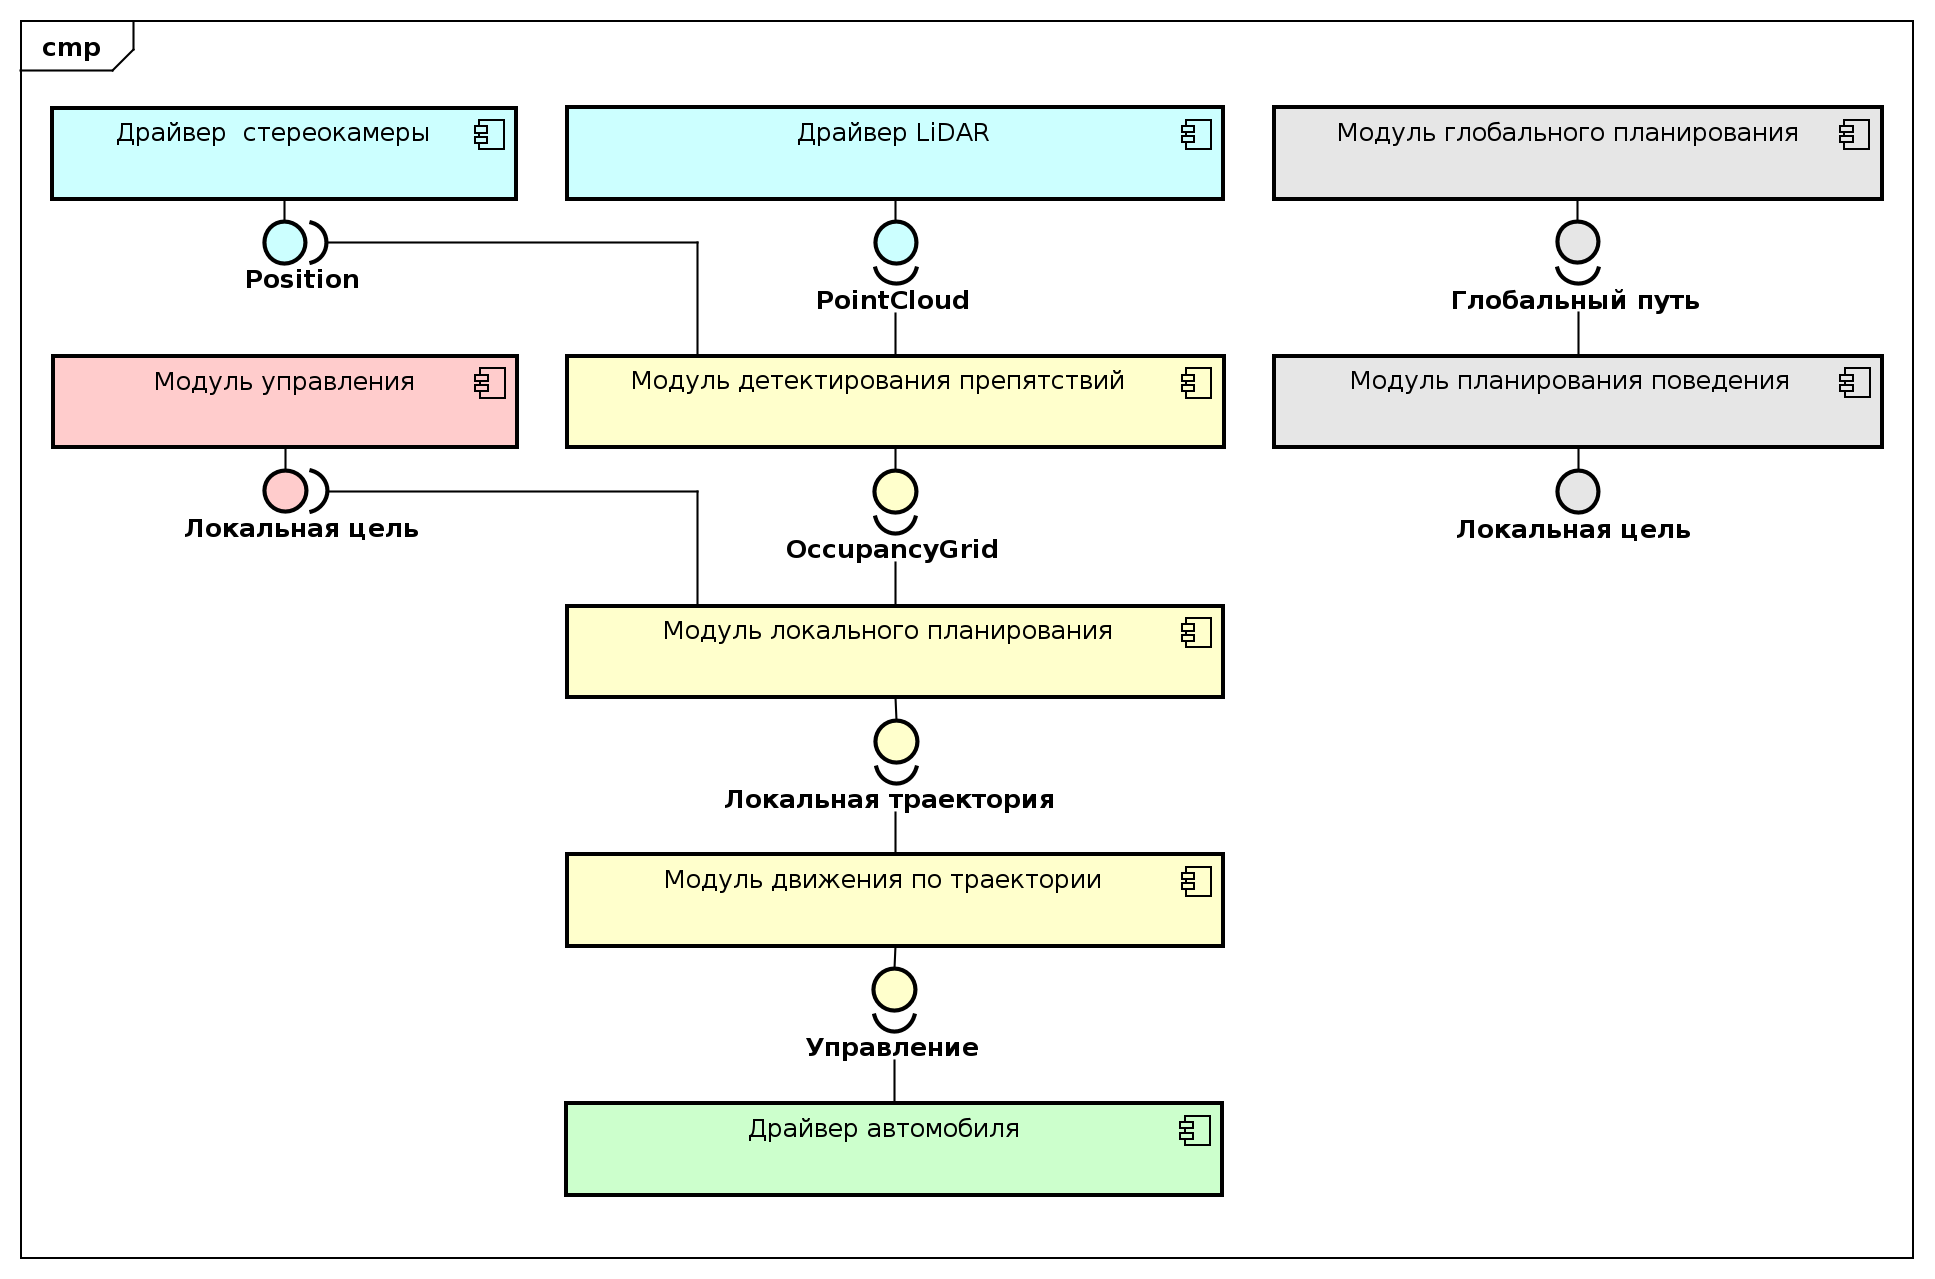
\includegraphics[width=\linewidth]{images/system_component_diagram}
      \caption{Диаграмма компонентов системы управления беспилотным автомобилем}
      \label{img:system_component_diagram}
  \end{figure}

Драйвер стереокамеры реализует работу со стереокамерой и алгоритм SLAM. Этот модуль предоставляет данные о текущем
положении и ориентации автомобиля в локальной системе координат. Драйвер LiDAR предоставляет облако точек, полученное
с LiDAR. Модуль детектирования препятствий осуществляет базовое детектирование препятствий в полученном облаке точек
и представляет информацию о них в виде т.н. Occupancy Grid. Occupancy Grid - это распространенный способ представления
информации о препятствиях в виде регулярной двухмерной сетки, каждая ячейка которой может быть в одном из трех
состояний: свободно, препятствие или неизвестно. Система управления беспилотным автомобилем в общем виде имеет модули
глобального планирования и планирования поведения, которые отвечают за построение глобальной траектории по дорожной
сети и принятие решений в соответствии с окружающей обстановкой и правилами дорожного движения, как было рассмотрено
в первой главе \ref{img:general_arch}. В рамках данной работы эти модули не рассматриваются и заменяются пользовательским
интерфейсом оператора, с помощью которого можно вручную указать локальную цель, вместо того, чтобы она задавалась
планировщиком поведения. На основании локальной цели, текущего положения автомобиля, полученного от модуля SLAM, и
инофрмации о препятствиях, полученных от модуля распознавания препятствий, модуль планирования локальной траектории
осуществляет планирование локальной траектории, которая позволит автомобилю достичь (если это возможно), поставленной
локальной цели. Сформированный локальным планировщиком путь поступает на вход регулятора с обратной связью, который
осуществляет управление исполнительными механизмами автомобиля, чтобы удерживать автомобиль на заданной траектории,
получая в качестве обратной связи текущее положение, ориентацию и скорость от модуля SLAM.

Разные этапы планирования требуют разное время и выполняются с различной частотой. \hl{TODO?}

\section{Проектирование подсистемы планирования локальной траектории}
Основной системой, разрабатываемой в рамках этой работы, является система планирования локальной траектории. Эта система
получает очередную цель от системы планирования поведения и осуществляет формирование оптимальной или близкой к нему
достижимой траектории для достижения этой цели. Достижимость подразумевает, что полученная траектория не приведет к
столкновению с известными препятствиями, с учетом габаритов препятствий и автомобиля, а также выполнима для автомобиля
с точки зрения его кинематики и динамики движения.

Существует большое количество различных алгоритмов планирования движения, ряд из которых был рассмотрен и проанализирован
в первой главе. Наиболее распространенными группами методов являются методы поиска на графах, включая различные
модификации, направленные на планирование достижимых для автомобиля путей, такие как методы решетки состояний
(state lattice), и методы интерполяции кривых. Первые являются более универсальными, и применяются в том числе для
планирования в неструктурированном окружении. Вторые больше ориентированы на планирование движения по дорогам, что
накладывает ряд ограничений, упрощающих задачу планирования движения.

В данной рамках данной работы реализуется метод планирования движения по дороге. \hl{Ну и почему?}

\subsection{A*}

\hl{TODO: написать про A*, что он не учитывал возможности машинки, что он прыгал туда-сюда, потом подвести к
полиномам, сказать, что у них непрерываные производные, и поэтому круто. Также сказать, что не самый топ, но сойдет}.

\subsection{Метод интерполяции кривых}
Первоначально был выбран подход и использованием интерполяции траектории кривыми \hl{ПОЧЕМУ?!}. За основу для
проектирования системы планирования локальной траектории был выбран метод, предложенный командой "Junior" Darpa
Urban Challenge \ref{img:junior_frenet_frame}, который был кратко рассмотрен в главе 1.

Для работы методы необходимы следующие входные данные:
\begin{itemize}
      \item опорная (рефернсная) траектория;
      \item локальная цель, описывающая требуемое положение и скорость автомобиля, эта точка должна
            лежать на опорной траектории;
      \item текущее состояние автомобиля (положение, скорость, ускорение);
      \item карта препятствий в формате Occupancy Grid.
\end{itemize}

Таким образом, планировщик поведения или, в случае данной работы, графический интерфейс оператора, должны предоставлять
опорную траекторию, помимо требуемого целевого состояния. Это требует дополнительной работы от планировшика поведения
и не позволяет сделать интерфейс локального планировщика полностью абстрактным, не зависящим от его реализации, потому
что не всем возможным реализациям требуется опорная траектория (например, алгоритмам на основе RRT она не требуется).
Тем не менее, это не является значительным препятствием. Опорная траектория при движении по непрерывному сегменту дороги
может быть реализована как центральная линия текущей полосы, по которой движется автомобиль. Это может быть определено
с помощью системы компьютерного зрения. Для более сложных ситуаций, например, перекрестков, подобная траектория может
быть реализована в виде сплайна, соединяющего соответствующие полосы двух пересекающихся дорог.

Планирование траектории осуществляется независимо для продольного движения вдоль опорной траектории и поперечного
движения. Планирование осуществляется в подвижной системе координат, движущейся по опорной траектории вместе с
автомобилем, как показано на рисунке \ref{img:frenet_frame}.

\begin{figure}[h]
      \centering
      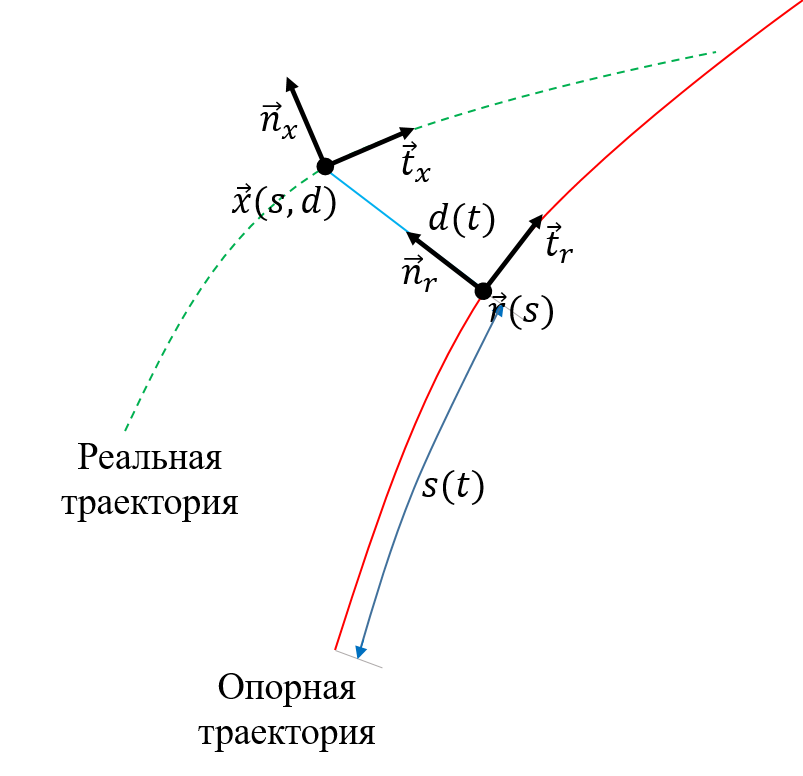
\includegraphics[]{images/frenet_frame}
      \caption{Диаграмма компонентов системы управления беспилотным автомобилем}
      \label{img:frenet_frame}
\end{figure}

Опорная траектория (изображена на рисунке красной линией) представлена натурально параметризованная кривая, где $s(t)$
~--- покрытая длина дуги в момент времени $t$. Положение автомобиля в глобальной системе координат обозначено
радиус-вектором $\vec{x}$. Этому положению автомобиля соответствует подвижная система координат $\vec{r}(s)$,
представляющая собой ортонормированный репер Френе, где $\vec{t}_r$ и $\vec{n}_r$ ~--- касательный и нормальный вектора
к опорной траектории соответственно. Таким образом, положение автомобиля в глобальной декартовой системе кординат
$(x, y)$ может быть представлено в подвижной системе координат как $(s, d)$, где $d$ - расстояние между автомобилем и
опорной траекторией.

Продольная и поперечная траектории движения ищутся в форме полиномов пятого порядка, соединяющие начальное состояние
(текущее состояние автомобиля, полученное от сенсоров) и целевое состояние (полученное от планировщика поведения или
графического интерфейса оператора). Первые и вторые производные этих
полиномов представляют собой зависимость скорости и ускорения автомобиля от времени, которые затем подаются в регулятор
с обратной связью наряду с пространственной траекторией движения, т.е. этот метод позволяет планировать не только
траекторию перемещения автомобиля, но и профиль скорости.

Задача состоит в том чтобы найти коэффициенты полинома, которые минимизируют некую функцию стоимости, используемую для
оценки траекторий. За основу для функции стоимости взят интеграл производной ускорения по времени $\dddot{s}$,
называемая рывок (jerk). Это является распространенным выбором функции стоимости во многих алгоритмов планирования
движения автомобилей. Ниже представлены интегралы для продольного и поперечного движения соответственно:
\begin{equation}
      J_s = \int_{t_0}^{t_1}{\dddot{s}(t)^2dt}
\end{equation}
\begin{equation}
      J_d = \int_{t_0}^{t_1}{\dddot{d}(t)^2dt}
\end{equation}

\noindent\begin{tabularx}{\linewidth}{lllX}
      где & $s(t), d(t)$ &~---& функция продольной и поперечной траекторий соответственно, \\
          & $t_0, t_1$   &~---& начальное и конечное время маневра соответственно. \\
\end{tabularx}

Такой выбор функции стоимости обоснован следующим:
\begin{itemize}
      \item минимизация количества и резкости маневров, совершаемых автомобилем (резкая траектория
            с большим количество маневров может быть получена в результате других алгоритмов
            планирования, таких как RRT), что повышает безопасность и экономичность движения;
      \item обеспечение комфорта пассажиров
\end{itemize}

В соответствии \cite{darpa_junior_frenet_origin} оптимальное решение, минимизирующее рывок, может быть найдено в форме
полиномов пятого порядка:
\begin{eqnarray}
      s(t)        =& a_0t^5   + a_1t^4 + a_2t^3 + a_3t^2 + a_4t + a_5 \\
      \dot{s}(t)  =& 5a_0t^4  + 4a_1t^3 + 3a_2t^2 + 2a_3t + a_4 \\
      \ddot{s}(t) =& 20a_0t^3 + 12a_1t^2 + 6a_2t + 2a_3
\end{eqnarray}

Помимо рывка, функция стоимости должна содержать ряд других членов:
\begin{itemize}
      \item отклонение конечной точки поперечной траектории от опорной траектории ~--- эта функция стоимости
            ухудшает оценку поперечных траекторий, которые не достигают заданной цели;
      \item отклонение конечной точки продольной траектории от покрытой длины дуги целевой точки ~--- эта функция
            стоимости ухудшает оценку продольных траекторий, которые не достигают заданной цели;
      \item отклонение первой производной продольной траектории от требуемой скорости ~--- эта функция стоимости
            ухудшает оценку продольных траекторий, которые не достигают заданной скорости;
      \item общее время совершения маневра ~--- эта функция стоимости ухудшает оценку слишком долгих траекторий.
\end{itemize}

Полная функция стоимости для поперечных траекторий:
\begin{equation}
      C_d = K_{dj} \int_{t_0}^{t_1}{\dddot{d}(t)^2dt} + K_d d(T)^2 + K_{dt} T
\end{equation}

Полная функция стоимости для продольных траекторий:
\begin{equation}
      C_s = K_{sj} \int_{t_0}^{t_1}{\dddot{s}(t)^2dt} + K_s (s(T) - S_1)^2 + K_v (\dot{s}(T) - \dot{S_1}) + K_{st} T
\end{equation}

\noindent\begin{tabularx}{\linewidth}{lllX}
      где & $K_{dj}, K_d, K_{dt}, K_{sj}, K_s, K_v, K_{st}$ &~---& весовые коэффициенты, \\
          & $S_1$                                           &~---& конечное (целевое) продольное состояние, \\
          & $T$                                             &~---& время выполнения маневра. \\
\end{tabularx}

Проблема заключается в том, что при оптимизации коэффициентов полинома необходимо учитывать ограничения. На траекторию
накладываются следующие ограничения:
\begin{itemize}
      \item максимальная продольная скорость,
      \item максимальное продольное ускорение (и замедление),
      \item максимальное поперечное ускорение,
      \item минимальная кривизна траектории,
      \item отсутствие пересечения с препятствиями.
\end{itemize}

Осуществление оптимизации коэффициентов полинома с учетом необходимости проверки на отсутствие пересечений с
препятствиями, которые представлены в виде Occupancy Grid. Поэтому вместо применения методов оптимизации применяется
широко распространенный в задачах планирования движения прием ~--- генерируется большой набор траекторий путем
варьирования конечного состояния $S1(T) = <s(t), \dot{s}(T), \ddot{s}(T)$ и времени $T$ в некотором диапазоне, а затем
производится выбор траектории с наименьшим значением функции стоимости среди тех, которые удовлетворяют ограничениями.

Имея начальное состояние $<s(0), \dot{s}(0), \ddot{s}(0)>$, конечное состояние $<\dot{s}(T), \ddot{s}(T), \ddot{s}(T)>$
и время совершения маневра $T$, можно рассчитать коэффициенты полинома, решив систему уравнений:
\begin{equation}
      \label{eq:solve_quintic}
      \begin{cases}
            \begin{array}
                  {lcl} a_5 = s(0) \\
                        a_4 = \dot{s}(0) \\
                        2a_3 = \ddot{s}(0) \\
                        a_0T^5   + a_1T^4 + a_2T^3 + a_3T^2 + a_4T + a_5 = s(T) \\
                        5a_0T^4  + 4a_1T^3 + 3a_2T^2 + 2a_3T + a_4 = \dot{s}(T)\\
                        20a_0T^3 + 12a_1T^2 + 6a_2T + 2a_3 = \ddot{s}(T)
            \end{array}
      \end{cases}
\end{equation}

На рисунке \ref{img:quntic_example} представлены графики примера продольной траектории, полученные путем решения
системы \ref{eq:solve_quintic}. В этом примере автомобиль тормозит с начальной скорости 15 м/с до полной остановки
за 7 секунд, преодолевая 60 метров.

\begin{figure}[h]
      \centering
      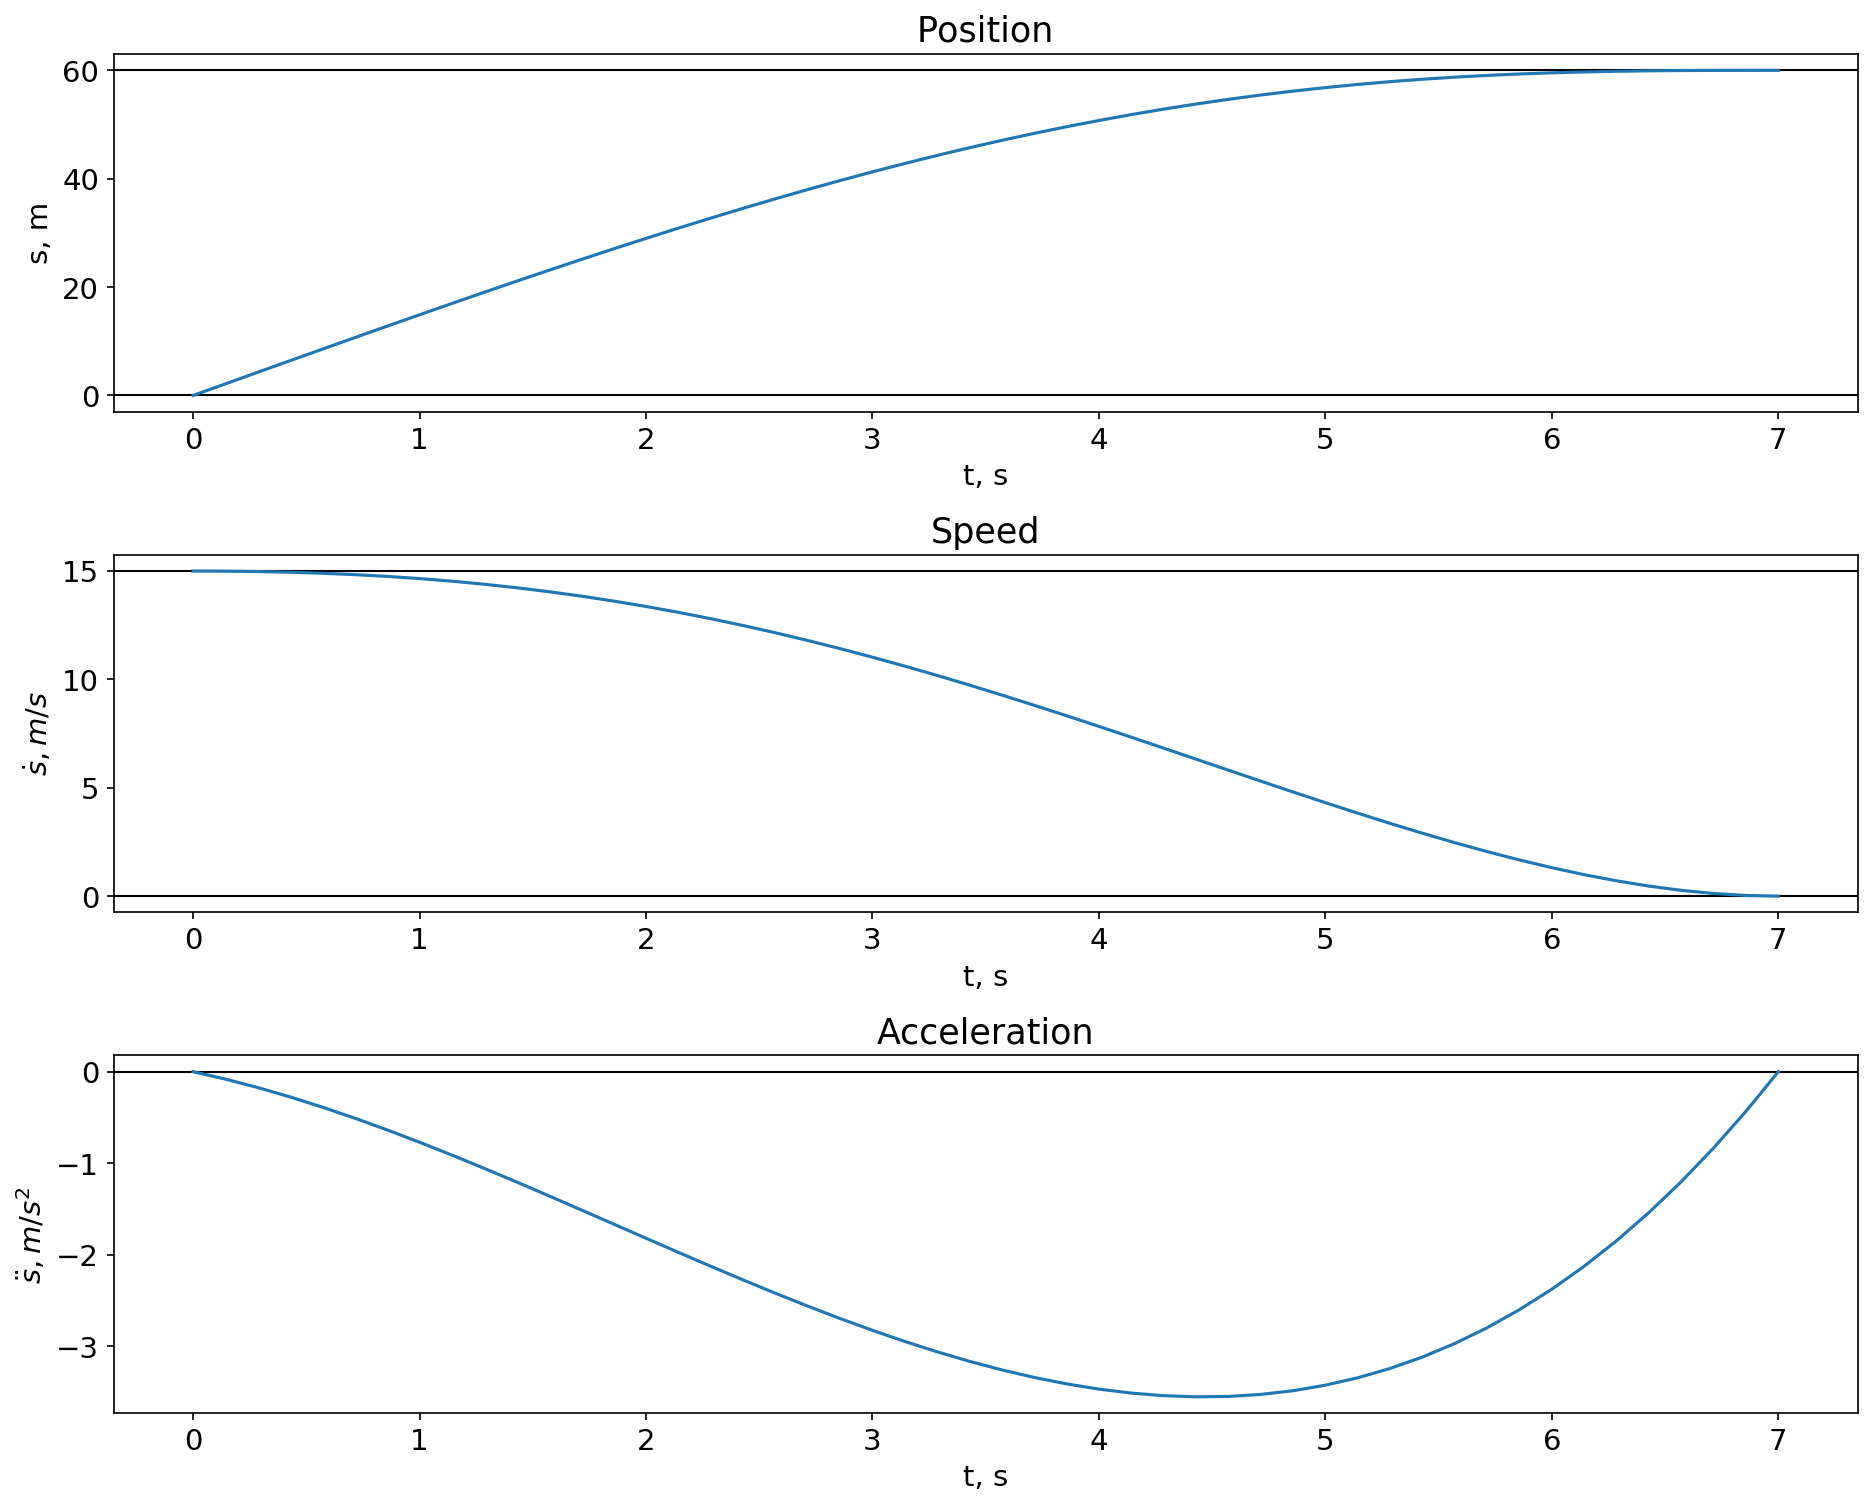
\includegraphics[width=\linewidth]{images/quintic_example}
      \caption{Пример траектории, описываемой полиномом пятого порядка}
      \label{img:quntic_example}
\end{figure}

\subsection{???}


\section{Проектирование подсистемы следования траектории}
